\newpage
\section{Faktorisieren und Ausmultiplizieren}
Durch das \textbf{Faktorisieren} oder Ausklammern wird eine Summe in ein Produkt umgeformt. Durch das \textbf{Ausmultiplizieren} wird ein Produkt in eine Summe umgeformt.

\begin{center}
  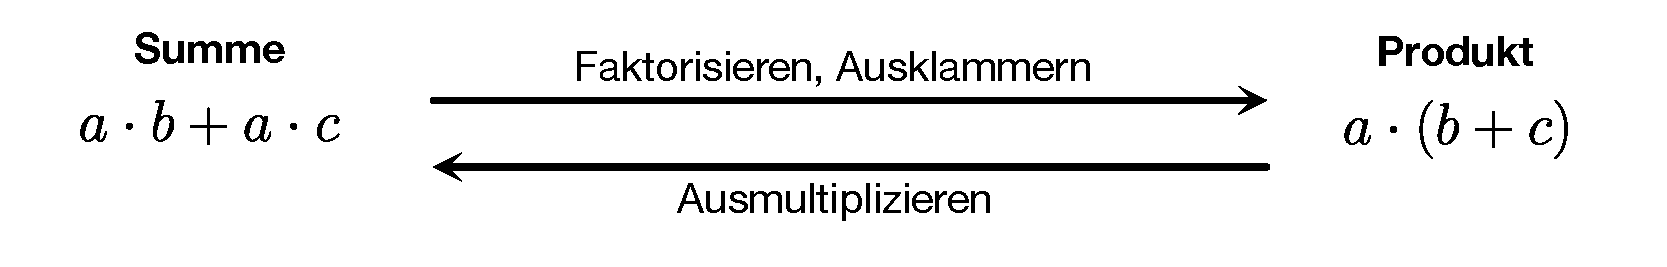
\includegraphics[width=.8\textwidth]{Faktorisieren.pdf}
\end{center}

Das Verwandeln eines Terms von einer Summe zu einem Produkt oder umgekehrt ist eine wichtige grundlegende Umformung, welche wir in der Mathematik immer wieder benötigen werden.

Es gibt ein paar Techniken, mit welchen Terme faktorisiert und ausmultipliziert werden können.

\subsection{Distributivgesetz}

Das Distributivgesetz für die Addition und Multiplikation lautet folgendermassen:
\[
  a\cdot(b+c) = a\cdot b + a\cdot c
\]

Das Distributivgesetz wird angewendet, um gemeinsame Faktoren aus Summanden auszuklammern. Dazu wird der grösste Faktor gesucht, welcher in allen Summanden vorkommt.

\begin{example}
  \textbf{Beispiele:} Faktorisieren Sie den Term $12x+16y$.
  \[
    4(3x+2y)
  \]
  Faktorisieren Sie den Term $4a^{2}+14a$.
  \[
    2a(a+7)
  \]
\end{example}

Auch ganze Terme können Faktoren sein, welche ausgeklammert werden können.

\begin{example}
  \textbf{Beispiel:} Faktorisieren Sie den Term $2(x+2y)-a(x+2y)$.

  Hier kommt der Faktor $(x+2y)$ in beiden Summanden vor und kann ausgeklammert werden:
  \[
    (x+2y)(2-a)
  \]
\end{example}

\subsection{Erste binomische Formel}
\[
  (a+b)^{2} = a^{2} + 2ab + b^{2}
\]
Die erste binomische berechnet die Fläche des Quadrats, das entsteht, wenn das Quadrat mit der Seitenlänge $a$ nach rechts und unten um $b$ vergrössert wird. Dazu wird links und unten ein Rechteck mit der Fläche $ab$ angesetzt. Unten rechts wird noch das Quadrat mit der Seitenlänge $b$ ergänzt.
\begin{center}
  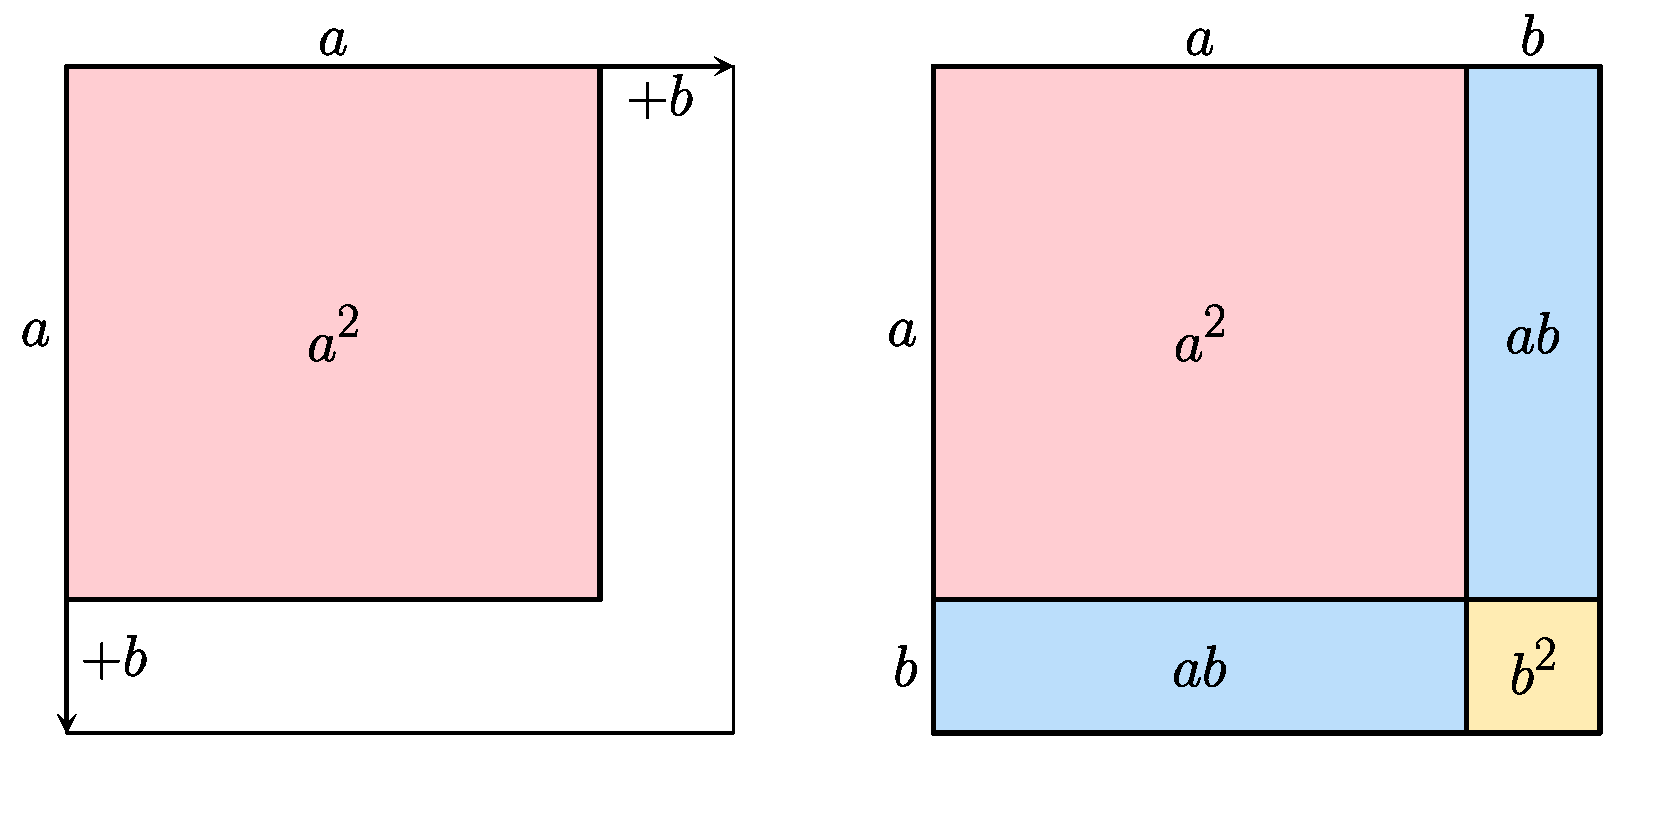
\includegraphics[width=.8\textwidth]{Binomische Formel 1.pdf}
\end{center}
Oft muss ein Term mit Hilfe anderer Regeln umgeformt und vorbereitet werden, bevor er mit einer binomischen Formel faktorisiert werden kann.
\begin{example}
  \textbf{Beispiel:} Faktorisieren Sie den Term $8u^{2}+2z^{2}+8uz$.

  \textbf{Lösung:} Zunächst wird $2$ ausgeklammert (Distributivgesetz):
  \[
    2\left(4u^{2}+z^{2}+4uz\right)
  \]
  Anschliessend werden die Summanden umgestellt (Kommutativgesetz):
  \[
    2\left(4u^{2}+4uz+z^{2}\right)
  \]
  Nun wird im mittleren Summanden der Faktor $2$ separat geschrieben:
  \[
    2\left(4u^{2}+2\cdot 2uz+z^{2}\right)
  \]
  Nun wird die erste binomische Formel angewendet mit $a=2u$ und $b=z$:
  \[
    2(2u+z)^{2}
  \]
\end{example}

\newpage

\subsection{Zweite binomische Formel}
\[
  (a-b)^{2} = a^{2} - 2ab + b^{2}
\]
Die zweite binomische Formel berechnet die Fläche des gelben Quadrats, welches entsteht, wenn vom Quadrat mit der Seitenlänge $a$ seitlich und unten ein Streifen der Breite $b$ abgeschnitten wird. Dabei wird zwei Mal ein Rechteck der Fläche $ab$ abgeschnitten, also $2ab$. Das Quadrat mit der Seitenlänge $b$ wurde dabei jedoch doppelt gezählt. Deshalb muss $b^{2}$ wieder addiert werden.
\begin{center}
  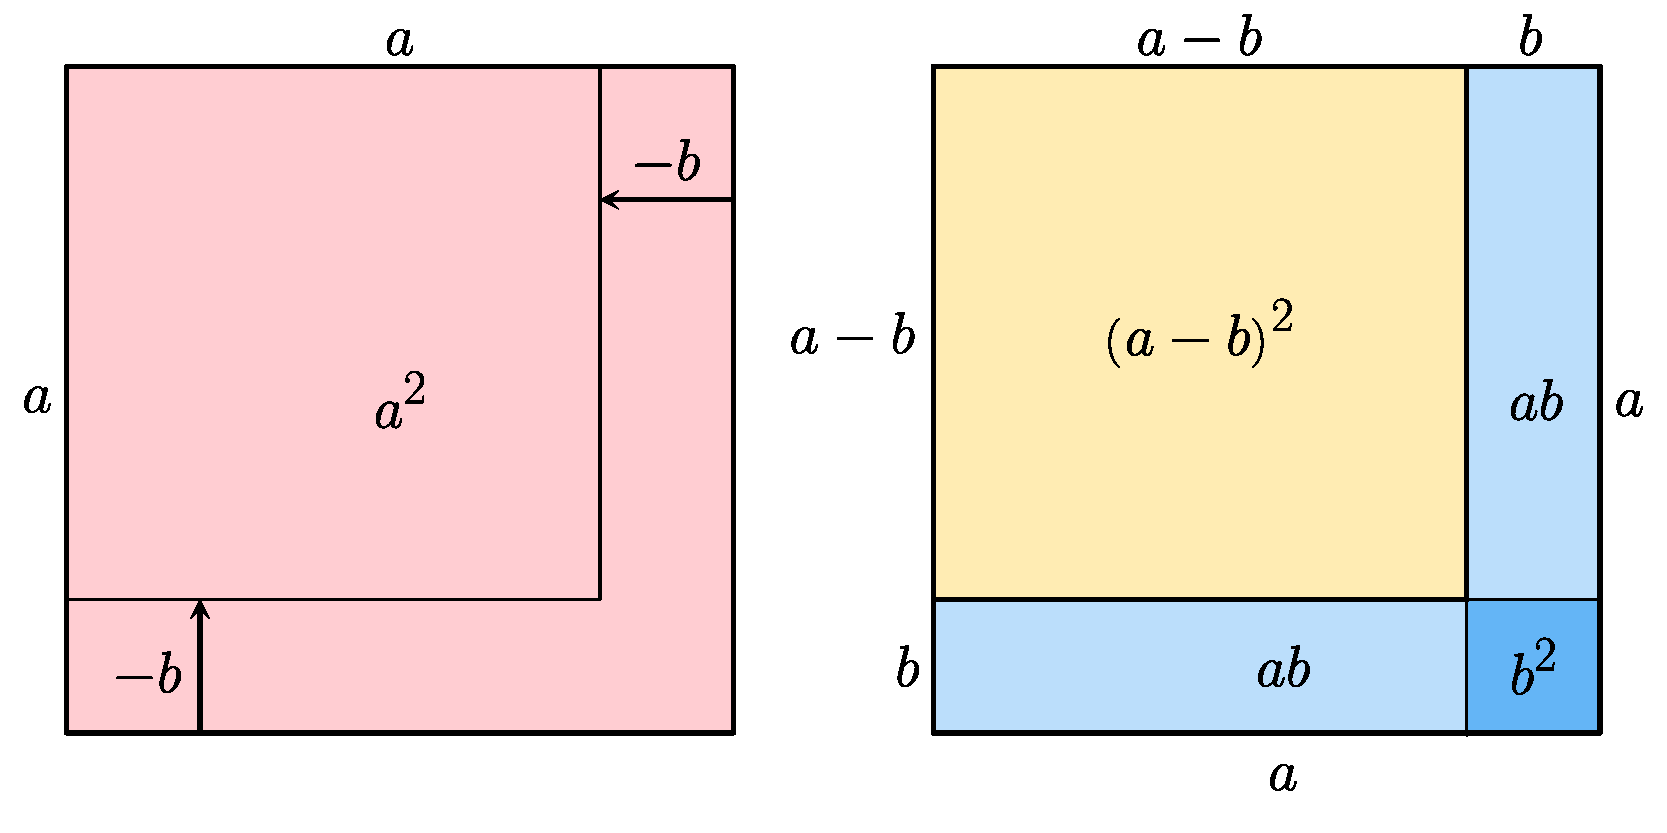
\includegraphics[width=.8\textwidth]{Binomische Formel 2.pdf}
\end{center}

\subsection{Dritte binomische Formel}
\[
  (a+b)(a-b) = a^{2} - b^{2}
\]
Die dritte binomische Formel berechnet die Fläche, welche entsteht, wenn aus dem Quadrat mit der Seitenlänge $a$ ein Quadrat mit der Seitenlänge $b$ ausgeschnitten wird. Die resultierende Fläche kann auseinander geschnitten und so arrangiert werden, dass ein Rechteck mit den Seitenlängen $a+b$ und $a-b$ entsteht.
\begin{center}
  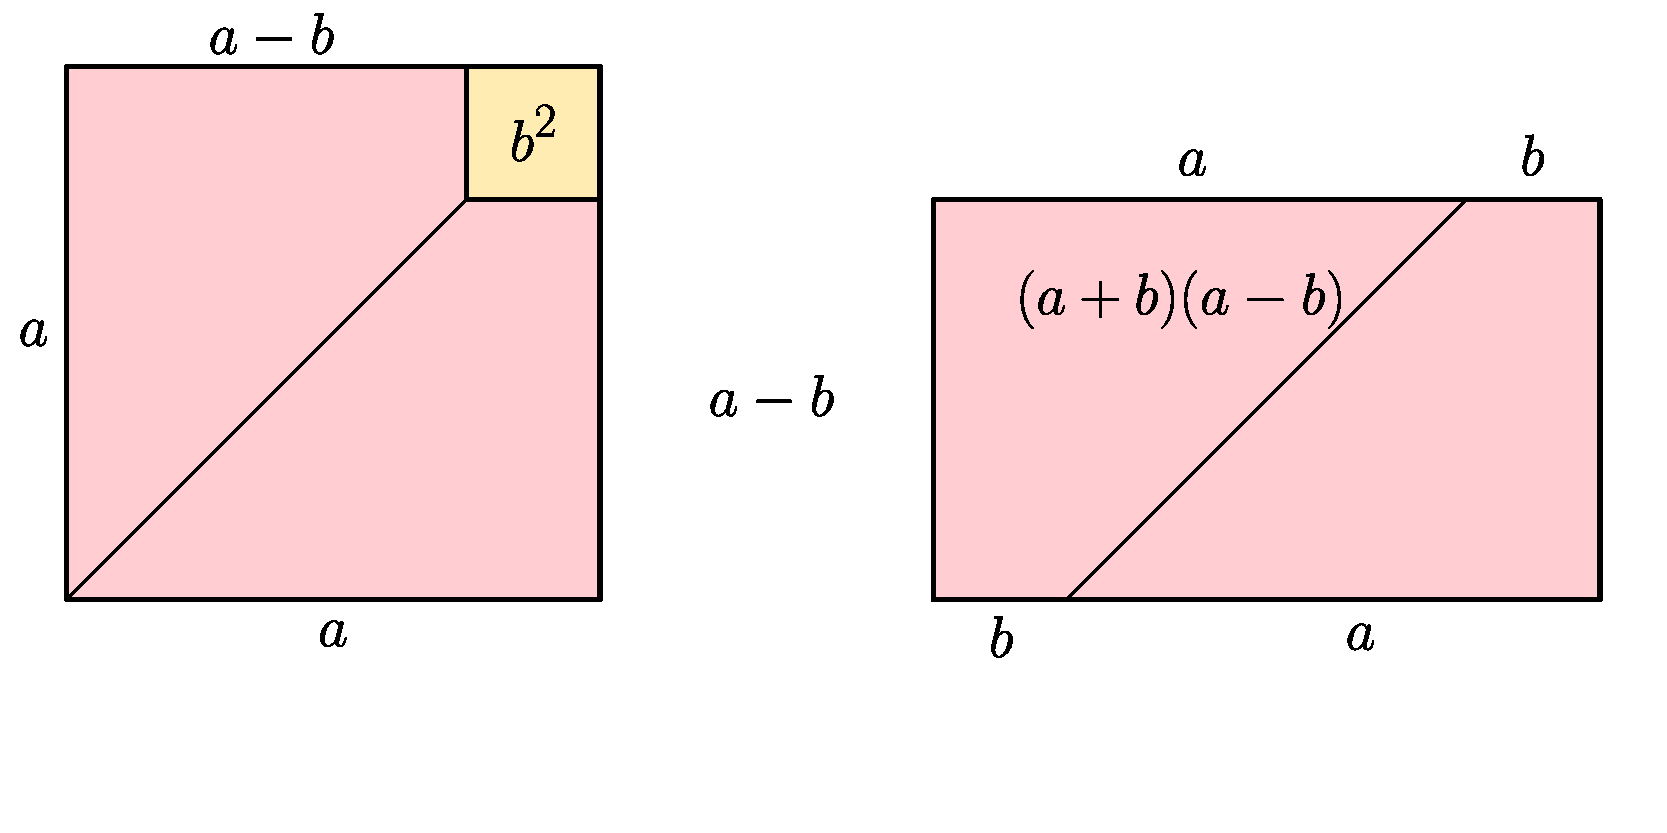
\includegraphics[width=.8\textwidth]{Binomische Formel 3.pdf}
\end{center}
